\documentclass[12pt]{article}

% Estilo oficial SBC: papel, margens, fontes, títulos e legendas.
\usepackage{sbc-template}
\usepackage{graphicx,url}
\usepackage[utf8]{inputenc}
\usepackage[T1]{fontenc}
\usepackage[brazil]{babel}
\usepackage{amsmath,amssymb,booktabs}
\usepackage[hidelinks]{hyperref}

% Citações autor-ano: (Autor, Ano), conforme os rótulos de sbc.bst.
\makeatletter
\renewcommand{\@cite}[2]{(#1\if@tempswa, #2\fi)}
\makeatother

\hypersetup{
	pdftitle={Transferência de arquivos via TCP e avaliação de desempenho no emulador CORE},
	pdfauthor={Henrique Campanha Garcia; Loren Pena Rodriguez Lorenzetto}
}

\sloppy
\title{Transferência de arquivos via TCP e avaliação de desempenho no emulador CORE}
% Autores informados pelo usuário; unidade confirmada no enunciado da disciplina.
\author{Henrique Campanha Garcia\inst{1},
	Loren Pena Rodriguez Lorenzetto\inst{1}}

\address{Instituto de Ciência e Tecnologia (ICT)\\
	Universidade Federal de São Paulo (UNIFESP)
	\email{henrique.garcia@unifesp.br, rafael.lorenzetto@unifesp.br}}


\begin{document}
\maketitle

\begin{abstract}
	This paper presents a C/Linux TCP file-transfer service and its evaluation using the CORE emulator. GET and PUT are tested with four file sizes, two network profiles and up to eight concurrent clients. The experiment completed 528 rounds and 2,288 transfers with matching SHA-256 hashes. Confidence intervals use rounds as the sampling unit. Large files approached the shared link capacity while response times increased with concurrency.
\end{abstract}

\begin{resumo}
	Este artigo apresenta um serviço de transferência de arquivos em C/Linux e sua avaliação no emulador CORE. GET e PUT foram avaliados com quatro tamanhos de arquivo, dois perfis de rede e até oito clientes simultâneos. Foram concluídas 528 rodadas e 2288 transferências com SHA-256 correto. Os intervalos de confiança usam a rodada como unidade amostral. Arquivos grandes se aproximaram da capacidade do enlace compartilhado, enquanto o tempo de resposta aumentou com a concorrência.
\end{resumo}

% ==========================================================
% 1. INTRODUÇÃO
% ==========================================================

\section{Introdução}
\label{sec:introducao}

A transferência de arquivos é uma das operações mais comuns em redes de computadores, sendo utilizada em diferentes aplicações que dependem da comunicação entre clientes e servidores. Para realizar essa comunicação, o protocolo \textit{Transmission Control Protocol} (TCP) oferece um fluxo confiável e ordenado de bytes. Entretanto, como o TCP não preserva os limites das mensagens enviadas pela aplicação, é necessário estabelecer um protocolo próprio para identificar comandos, delimitar os dados transmitidos e determinar o término de cada operação \cite{tcp}.

Além da comunicação, o atendimento simultâneo de múltiplos clientes representa um aspecto importante no desenvolvimento de servidores. À medida que o número de conexões aumenta, recursos como processamento, memória e capacidade de transmissão da rede passam a ser compartilhados, podendo afetar o desempenho das operações. Nesse contexto, técnicas de programação paralela, como o OpenMP, permitem organizar o processamento concorrente das requisições.

Neste trabalho, foi desenvolvida uma aplicação cliente-servidor em linguagem C, utilizando sockets TCP no ambiente Linux. A aplicação implementa as operações GET e PUT, responsáveis, respectivamente, pelo recebimento e envio de arquivos, com suporte à transferência de dados binários e ao atendimento simultâneo de múltiplos clientes por meio do OpenMP.

Após a implementação, foi realizada uma avaliação de desempenho utilizando o emulador de redes CORE. Os experimentos consideraram dois perfis de rede, quatro tamanhos de arquivo e diferentes níveis de concorrência, com até oito clientes simultâneos. Para cada configuração, foram analisados o tempo de resposta e a vazão útil das operações, além da integridade dos arquivos transferidos.

O objetivo principal é avaliar como o tamanho dos arquivos, a quantidade de clientes concorrentes e as condições de vazão e latência da rede influenciam o desempenho da aplicação. Dessa forma, busca-se compreender o comportamento do serviço em diferentes condições de comunicação e identificar possíveis limitações relacionadas ao compartilhamento dos recursos disponíveis.

% ==========================================================
% 2. IMPLEMENTAÇÃO DO CLIENTE-SERVIDOR
% ==========================================================

\section{Implementação do Cliente-Servidor}
\label{sec:implementacao}

A aplicação foi desenvolvida em C, utilizando sockets TCP para a comunicação entre cliente e servidor. O atendimento simultâneo de múltiplos clientes foi implementado com OpenMP. Durante a revisão do código, foram corrigidos problemas relacionados ao controle de conexões, à sobrescrita de arquivos e ao tratamento de respostas. Os arquivos originais foram preservados para comparação.

\subsection{Protocolo e Tratamento de Erros}

Foi definido um protocolo simples baseado em comandos ASCII terminados por quebra de linha (\texttt{LF}). Na operação \texttt{GET}, o cliente solicita um arquivo e o servidor responde com \texttt{OK tamanho}, seguido dos dados, ou com \texttt{ERR} em caso de falha. No \texttt{PUT}, o cliente informa o nome e o tamanho do arquivo, aguarda a resposta \texttt{READY} e inicia a transferência, recebendo \texttt{OK} ao final.

A aplicação suporta arquivos binários de até 1 GiB, utilizando nomes sem espaços ou caminhos de diretórios. As rotinas de comunicação tratam envios e recebimentos parciais, interrupções por \texttt{EINTR} e desconexões inesperadas. Também foram configurados timeouts de comunicação de 15 segundos para evitar bloqueios indefinidos.

\subsection{Concorrência e Sobrescrita}

O servidor utiliza OpenMP \cite{openmp} para atender até oito clientes simultaneamente. Cada conexão é processada separadamente, evitando interferência entre as operações. Quando a capacidade de atendimento é atingida, novas conexões podem aguardar na fila do sistema operacional.

Para evitar a perda de arquivos durante transferências interrompidas, as operações \texttt{PUT} gravam os dados em arquivos temporários. Após o recebimento completo, o arquivo é renomeado para o destino, substituindo a versão anterior. O mesmo procedimento é utilizado pelo cliente durante o \texttt{GET}.

Essa abordagem permite a substituição atômica dos arquivos durante a execução normal. Entretanto, não garante a persistência dos dados em caso de falha de energia, pois não utiliza \texttt{fsync()}.

\subsection{Verificação da Implementação}

A aplicação foi compilada com GCC, utilizando C11 e OpenMP. Foram executados 11 testes de integração, repetidos com uma camada de interposição de sockets para simular envios e recebimentos parciais e interrupções \texttt{EINTR}.

Os testes incluíram arquivos de 0 bytes a 4 MiB, operações GET e PUT, sobrescrita, desconexões, comandos inválidos e verificação de integridade por SHA-256. A concorrência foi avaliada com oito clientes simultâneos, incluindo transferências para o mesmo destino.

Todos os testes foram concluídos com sucesso, tanto na execução convencional quanto na execução com operações parciais simuladas.

% ==========================================================
% 3. AMBIENTE EXPERIMENTAL
% ==========================================================

\section{Ambiente Experimental e Topologia CORE}
\label{sec:ambiente}

Os experimentos foram realizados utilizando o emulador de redes CORE \cite{core}, versão 9.2.0, executado em um contêiner Docker sobre Ubuntu 22.04/WSL2. O ambiente utilizou Python 3.10, e os nós emulados compartilharam os recursos computacionais da máquina hospedeira.

A topologia, apresentada na Figura~\ref{fig:topologia}, foi composta por oito clientes, um servidor, dois roteadores e três switches. Foram utilizadas três sub-redes: 10.10.0.0/24 para os clientes, 10.20.0.0/24 para o núcleo e 10.30.0.0/24 para o servidor, que atende na porta 8080. A comunicação entre as redes foi realizada por meio de roteamento estático.

\begin{figure}[!htbp]
	\centering
	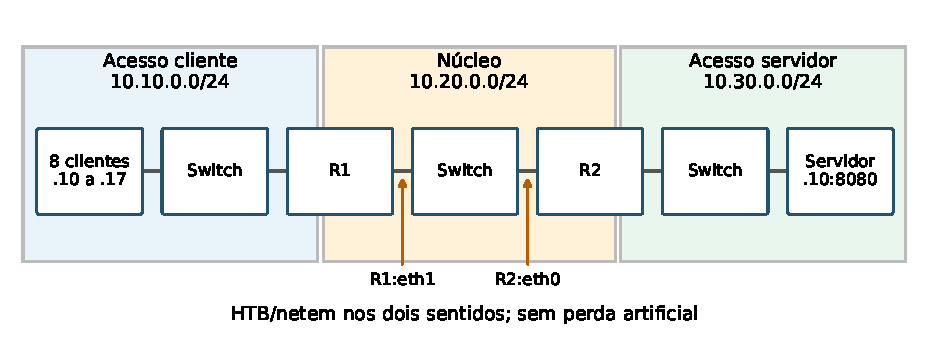
\includegraphics[width=\linewidth]{figuras/topologia.pdf}
	\caption{Topologia utilizada no CORE, com o enlace de gargalo entre os roteadores R1 e R2.}
	\label{fig:topologia}
\end{figure}

\subsection{Perfis e Validação da Rede}

Foram definidos dois perfis de rede, variando a vazão e a latência do enlace de gargalo. O perfil A foi configurado com 100 Mbps e 5 ms de atraso por direção, enquanto o perfil B utilizou 20 Mbps e 30 ms. Dessa forma, os RTTs nominais foram de 10 ms e 60 ms, respectivamente. Os valores foram escolhidos para representar diferentes condições de acesso, sem corresponder necessariamente a uma tecnologia específica.

As limitações foram aplicadas utilizando HTB para controle de vazão e netem para configuração do atraso, sem introdução de perda artificial de pacotes. Também foram desativados os mecanismos TSO, GSO e GRO, mantendo o algoritmo de controle de congestionamento TCP CUBIC.

Para validar a configuração, foram realizados testes com ping, traceroute e iperf3 \cite{iperf}. O ping verificou o RTT entre cliente e servidor, enquanto o traceroute confirmou a passagem pelos roteadores intermediários. O iperf3 foi utilizado para medir a vazão nos dois sentidos, permitindo comparar os valores observados com os parâmetros configurados.

Os resultados são apresentados na Tabela~\ref{tab:validacao}. Não foram observadas perdas nos testes de ping, e o traceroute confirmou o caminho esperado entre cliente e servidor.

% Valores transcritos dos dados entregues; não editar manualmente.
\begin{table}[htbp]
	\centering
	\caption{Validação do caminho cliente--servidor nos dois perfis.}
	\label{tab:validacao}
	\begin{tabular}{lrrrr}
		\toprule
		Perfil & RTT (ms) & Ida (Mbps) & Volta (Mbps) & Perdas \\
		\midrule
		A & 11,817 & 95,348 & 94,995 & 0/10 \\
		B & 60,707 & 19,206 & 19,085 & 0/10 \\
		\bottomrule
	\end{tabular}
\end{table}


% ==========================================================
% 4. METODOLOGIA
% ==========================================================

\section{Metodologia dos experimentos}
\label{sec:metodologia}

\subsection{Fatores e Repetições}

Foram utilizados quatro tamanhos de arquivos binários: 32 e 256 KiB, representando imagens de aplicações Web, e 1 e 4 MiB, representando anexos e arquivos de armazenamento em nuvem. Os arquivos foram gerados de forma determinística, permitindo a reprodução dos testes.

A matriz experimental considerou dois perfis de rede, duas operações (GET e PUT), quatro tamanhos de arquivo e três níveis de concorrência (1, 4 e 8 clientes). Cada configuração foi repetida 11 vezes, totalizando $2 \times 2 \times 4 \times 3 \times 11 = 528$ rodadas e 2288 transferências. A ordem foi embaralhada com a semente 20261105, reduzindo possíveis efeitos da sequência de execução.

Antes da coleta principal, foram realizados testes piloto, que não foram incluídos na análise. Não houve remoção de valores extremos nem limpeza do cache de arquivos entre as execuções.

\subsection{Concorrência, Tempo e Vazão}

Cada cliente foi executado como um processo independente em um nó do CORE. Para sincronizar as requisições, os processos utilizaram uma barreira baseada no relógio monotônico, com início programado 150 ms à frente.

O tempo de resposta foi medido com \texttt{CLOCK\_MONOTONIC}, incluindo conexão, negociação, transferência e conclusão da operação. No PUT, a medição termina após a confirmação do servidor; no GET, após a gravação e publicação do arquivo local. A geração dos dados e a verificação SHA-256 ficaram fora da medição. Foram utilizados limites de execução de 55 segundos por cliente e 60 segundos por comando do nó.

A vazão útil individual foi calculada por:

\begin{equation}
	G = \frac{8B}{10^6 T}
	\label{eq:vazao}
\end{equation}

\noindent em que $G$ representa a vazão em Mbps, $B$ o tamanho do arquivo em bytes e $T$ o tempo de resposta em segundos. A vazão agregada considera a soma dos bytes transferidos dividida pelo intervalo entre o início da primeira operação e a conclusão da última.

\subsection{Integridade e Coleta de Dados}

Para cada transferência, foram registrados perfil de rede, operação, tamanho do arquivo, concorrência, repetição, tempo de resposta, vazão, bytes transferidos, status e hashes de integridade.

A integridade foi verificada utilizando SHA-256, comparando os arquivos de origem e destino. Nas operações PUT, cada cliente utilizou um nome remoto diferente para evitar conflitos de escrita.

Os resultados foram armazenados em CSV, com um mecanismo de checkpoint para permitir a retomada dos experimentos sem duplicar rodadas. A retomada foi testada após duas execuções, e apenas rodadas completas e confirmadas foram consideradas na análise. O mecanismo não foi avaliado contra corrupção de arquivos ou falhas de energia.

\subsection{Tratamento Estatístico}

Como os clientes de uma mesma rodada compartilham os recursos da rede e do servidor, a rodada foi utilizada como unidade de repetição para estimar a incerteza das medições.

Foram calculadas média, mediana e desvio padrão. Para o tempo de resposta e a vazão individual, calculou-se inicialmente a média dos clientes de cada rodada e, em seguida, o intervalo de confiança de 95\% entre as 11 médias, utilizando a distribuição t de Student:

\begin{equation}
	IC_{95\%} = \bar{x} \pm
	t_{0{,}975;10}\frac{s}{\sqrt{11}}
	\label{eq:intervalo}
\end{equation}

\noindent em que $\bar{x}$ é a média das rodadas, $s$ o desvio padrão amostral entre elas e $t_{0{,}975;10}$ o valor crítico da distribuição t com 10 graus de liberdade.

Para a mediana, foram utilizados intervalos de confiança obtidos por bootstrap com 3000 reamostragens de rodadas completas, preservando o agrupamento dos clientes. A vazão agregada foi analisada por rodada, e as taxas de sucesso consideraram todas as transferências.

% ==========================================================
% 5. RESULTADOS
% ==========================================================

\section{Resultados e Análise Estatística}
\label{sec:resultados}

A campanha experimental foi realizada em 5 de novembro de 2026, entre 17:05 e 17:22 UTC. Foram concluídas 528 rodadas e 2288 transferências, todas com sucesso e integridade confirmada por SHA-256. Cada uma das 48 configurações teve 11 repetições, sem exclusão de observações.

Nas rodadas com múltiplos clientes, foi confirmada a sobreposição temporal das operações, com desvio máximo de 2,038 ms entre os inícios e sobreposição mínima de 33,313 ms. Esses resultados, juntamente com os testes de concorrência, confirmam o atendimento simultâneo das requisições.

A Tabela~\ref{tab:tempos} apresenta as estatísticas de tempo de resposta para arquivos de 4 MiB, enquanto a Figura~\ref{fig:tempo} mostra os tempos médios para todos os tamanhos. Os resultados completos, incluindo os intervalos de confiança, estão disponíveis nos arquivos CSV.

% Valores transcritos dos dados entregues; não editar manualmente.
\begin{table}[htbp]
	\centering
	\caption{Tempo de resposta para 4 MiB, em segundos. O IC da média usa 11 rodadas; mediana e
		desvio padrão (DP) descrevem as observações individuais.}
	\label{tab:tempos}
	\begin{tabular}{llcrrrr}
		\toprule
		Perfil & Op. & $N$ & Média & Mediana & DP & IC 95\% \\
		\midrule
		A & GET & 1 & 0,396 & 0,397 & 0,001 & [0,396; 0,397] \\
		A & GET & 4 & 1,301 & 1,333 & 0,138 & [1,264; 1,339] \\
		A & GET & 8 & 2,602 & 2,679 & 0,264 & [2,502; 2,702] \\
		A & PUT & 1 & 0,411 & 0,411 & 0,003 & [0,409; 0,413] \\
		A & PUT & 4 & 1,324 & 1,382 & 0,146 & [1,273; 1,375] \\
		A & PUT & 8 & 2,543 & 2,565 & 0,270 & [2,495; 2,591] \\
		B & GET & 1 & 2,024 & 2,024 & 0,001 & [2,023; 2,024] \\
		B & GET & 4 & 6,626 & 7,101 & 0,734 & [6,341; 6,912] \\
		B & GET & 8 & 13,030 & 13,697 & 1,211 & [12,922; 13,138] \\
		B & PUT & 1 & 2,102 & 2,085 & 0,055 & [2,065; 2,139] \\
		B & PUT & 4 & 6,380 & 6,495 & 0,876 & [6,159; 6,602] \\
		B & PUT & 8 & 13,422 & 13,787 & 0,776 & [13,333; 13,510] \\
		\bottomrule
	\end{tabular}
\end{table}


\begin{figure}[!htbp]
	\centering
	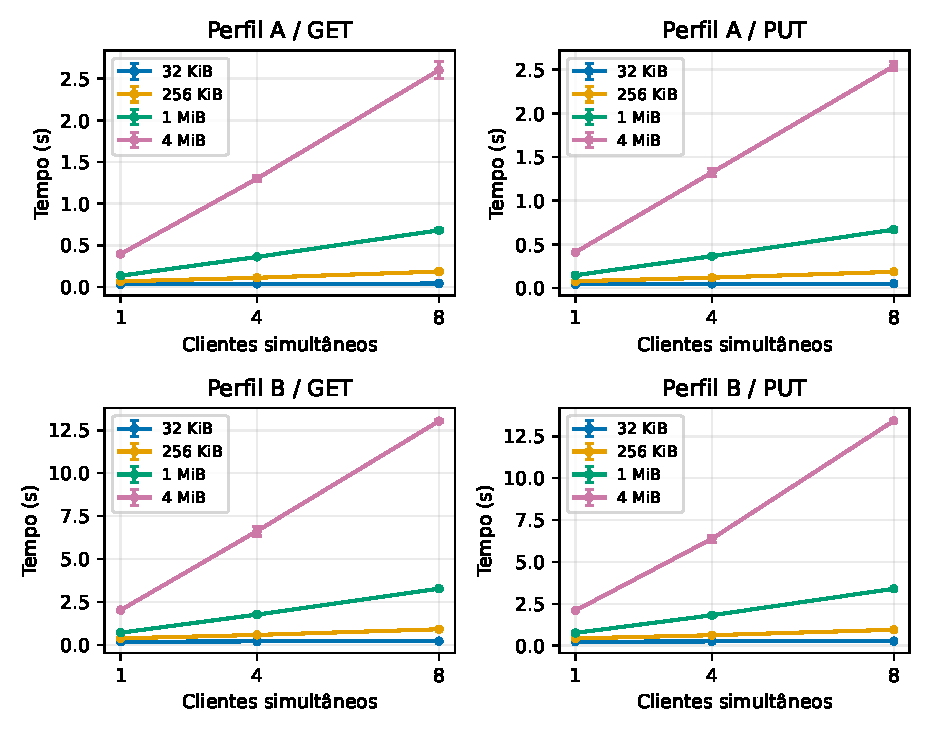
\includegraphics[width=\linewidth]{figuras/tempo_resposta.pdf}
	\caption{Tempo médio de resposta por operação, perfil e concorrência, com IC de 95\% entre rodadas.}
	\label{fig:tempo}
\end{figure}

As Figuras~\ref{fig:individual} e~\ref{fig:agregada} apresentam, respectivamente, a vazão útil individual e a vazão agregada. Para arquivos de 4 MiB e oito clientes, a vazão agregada ficou próxima de 94 Mbps no perfil A e 19 Mbps no perfil B. Entre quatro e oito clientes, o ganho agregado foi de aproximadamente 1,4\% a 2,1\%, dependendo da operação e do perfil.

\begin{figure}[!htbp]
	\centering
	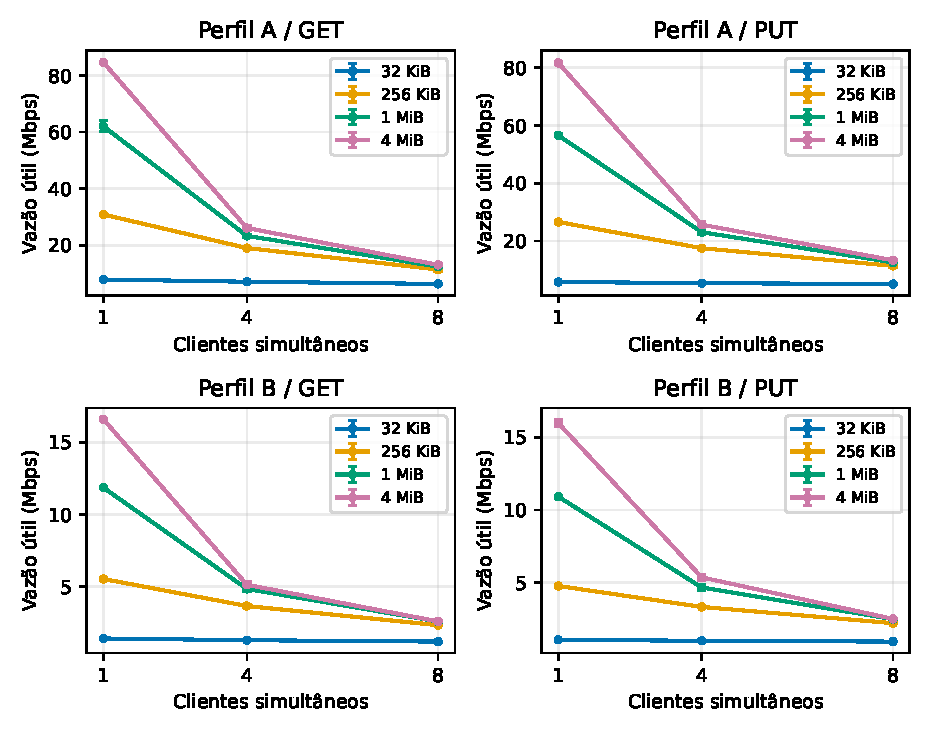
\includegraphics[width=\linewidth]{figuras/vazao_individual.pdf}
	\caption{Vazão útil individual por perfil e concorrência, com IC de 95\% entre rodadas.}
	\label{fig:individual}
\end{figure}

\begin{figure}[!htbp]
	\centering
	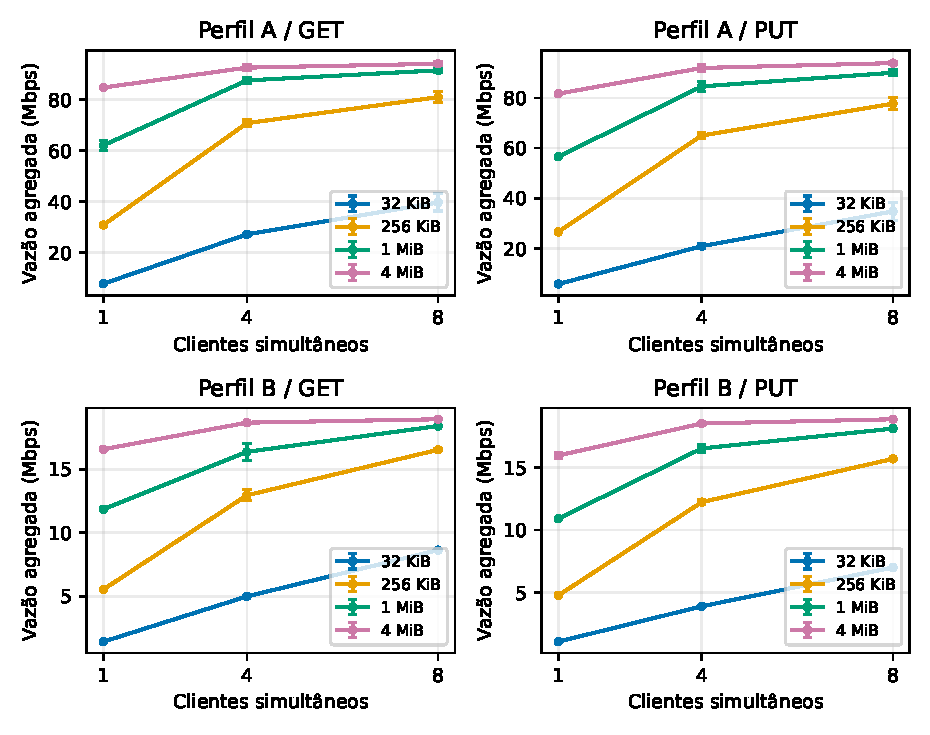
\includegraphics[width=\linewidth]{figuras/vazao_agregada.pdf}
	\caption{Vazão agregada por rodada, com IC de 95\%.}
	\label{fig:agregada}
\end{figure}

Para arquivos de 32 KiB e um cliente, o GET apresentou tempos próximos de 0,033 s no perfil A e 0,185 s no B. No PUT, os tempos foram de 0,045 s e 0,245 s, respectivamente. A Tabela~\ref{tab:comparacoes} apresenta comparações entre os cenários extremos de tamanho e concorrência.

% Valores transcritos dos dados entregues; não editar manualmente.
\begin{table}[htbp]
	\centering
	\caption{Razões entre médias de tempo de resposta. Valores descritivos, sem teste de
		hipótese ou intervalo específico para as razões.}
	\label{tab:comparacoes}
	\begin{tabular}{rrrrrr}
		\toprule
		KiB & $N$ & PUT/GET A & PUT/GET B & B/A GET & B/A PUT \\
		\midrule
		32 & 1 & 1,343 & 1,325 & 5,543 & 5,469 \\
		32 & 8 & 1,222 & 1,266 & 5,202 & 5,387 \\
		4096 & 1 & 1,036 & 1,039 & 5,104 & 5,117 \\
		4096 & 8 & 0,977 & 1,030 & 5,007 & 5,279 \\
		\bottomrule
	\end{tabular}
\end{table}


Por fim, a Figura~\ref{fig:distribuicao} apresenta a distribuição dos tempos individuais para arquivos de 4 MiB, enquanto a Figura~\ref{fig:cdf} mostra a distribuição acumulada empírica (CDF) para um e oito clientes.

\begin{figure}[!htbp]
	\centering
	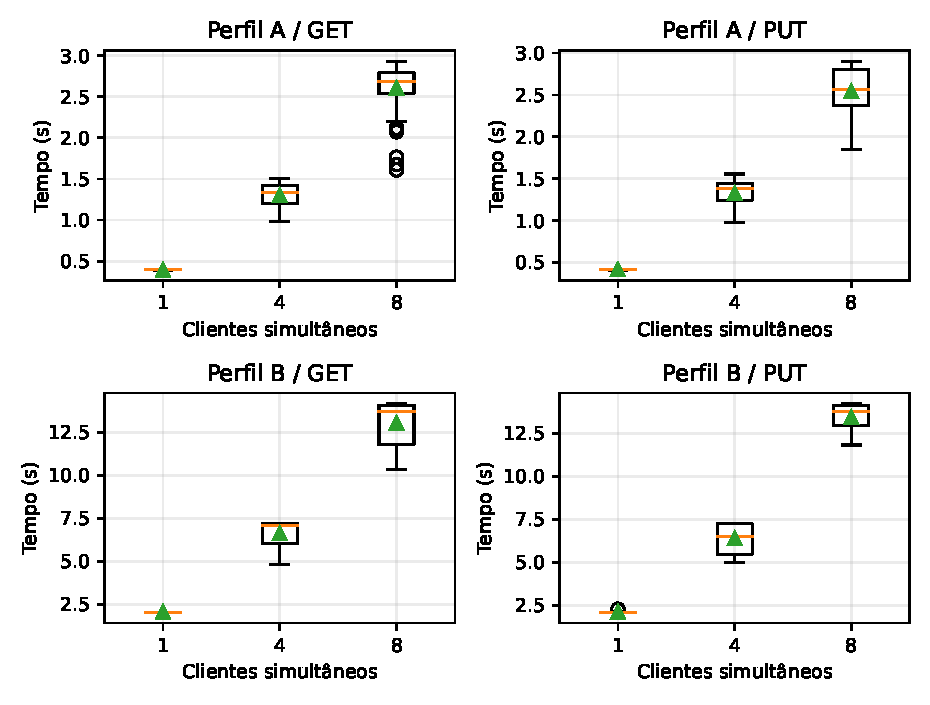
\includegraphics[width=\linewidth]{figuras/distribuicao.pdf}
	\caption{Distribuição dos tempos individuais para arquivos de 4 MiB, com médias indicadas por triângulos.}
	\label{fig:distribuicao}
\end{figure}

\begin{figure}[!htbp]
	\centering
	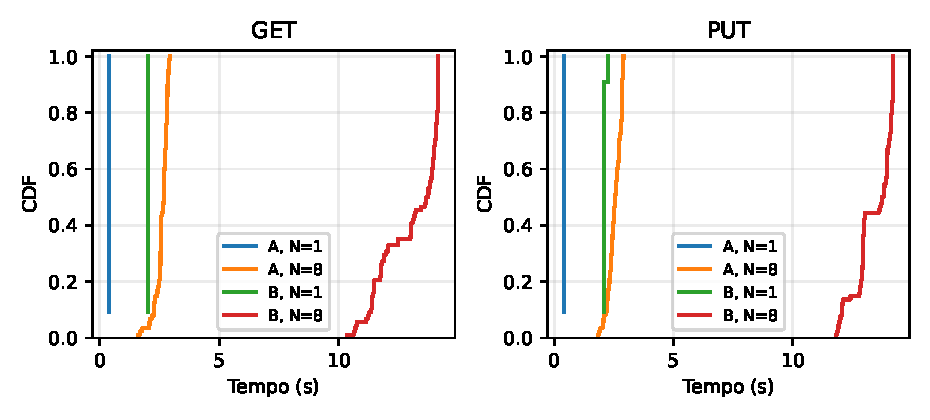
\includegraphics[width=\linewidth]{figuras/cdf.pdf}
	\caption{CDF empírica dos tempos de resposta para arquivos de 4 MiB, comparando os perfis e níveis de concorrência.}
	\label{fig:cdf}
\end{figure}


% ==========================================================
% 6. DISCUSSÃO DOS RESULTADOS
% ==========================================================

\section{Discussão dos Resultados}
\label{sec:discussao}

Os resultados indicam que o aumento da concorrência eleva o tempo de resposta individual, enquanto a vazão agregada apresenta ganhos cada vez menores. Para arquivos de 4 MiB, o GET apresentou tempos entre aproximadamente 0,396 s e 2,602 s no perfil A, e entre 2,024 s e 13,030 s no perfil B. No PUT, os valores variaram de 0,411 s a 2,543 s em A e de 2,102 s a 13,422 s em B.

Esse comportamento é compatível com a saturação do enlace de gargalo, já que sua capacidade passa a ser compartilhada entre mais clientes. Entretanto, os três níveis de concorrência avaliados não permitem determinar um ponto exato de saturação.

As diferenças entre GET e PUT também dependem das etapas de cada operação. O PUT aguarda a autorização para envio e a confirmação final, enquanto o GET recebe o cabeçalho e realiza a gravação local. Essas diferenças são mais perceptíveis em arquivos pequenos, mas os resultados não permitem afirmar que uma operação seja sempre mais rápida.

O perfil B apresentou tempos maiores devido à combinação de menor vazão e maior latência. Como esses dois parâmetros foram alterados simultaneamente, não é possível determinar isoladamente a contribuição de cada um. Em arquivos maiores, a capacidade do enlace exerce maior influência, enquanto arquivos pequenos são mais sensíveis aos custos fixos de comunicação.

\subsection{Limitações}

Os experimentos foram realizados em um ambiente CORE sobre WSL2 e Docker, no qual os nós compartilham os recursos da máquina hospedeira. Além disso, os perfis utilizaram atrasos fixos, sem introdução de jitter ou perda artificial de pacotes.

Não foram monitorados continuamente o uso de CPU, disco e filas durante cada rodada, o que limita a identificação das causas de variações individuais. Também não foram avaliados TLS, autenticação ou a durabilidade dos arquivos após falhas de energia.

Por fim, as 11 repetições por configuração permitem estimar a variabilidade observada, mas não eliminam possíveis efeitos temporais. A ausência de falhas na campanha também não garante que o sistema esteja livre de erros em outras condições.


% ==========================================================
% 7. CONCLUSÕES
% ==========================================================

\section{Conclusões}
\label{sec:conclusoes}

O trabalho apresentou a implementação de uma aplicação cliente-servidor TCP em C, com operações GET e PUT e atendimento concorrente utilizando OpenMP. Os testes verificaram a transferência de arquivos binários, sobrescrita, tratamento de erros e atendimento simultâneo de até oito clientes.

Na avaliação realizada com o CORE, foram concluídas 528 rodadas e 2288 transferências, todas com integridade confirmada. Os resultados mostraram que o aumento da concorrência pode elevar significativamente o tempo de resposta individual, enquanto a vazão agregada se aproxima da capacidade do enlace de gargalo.

Os códigos, dados experimentais e arquivos de configuração foram organizados no repositório do projeto, permitindo a reprodução dos testes e das análises realizadas.


% ==========================================================
% NOTA SOBRE O USO DE IA
% ==========================================================

\section*{Nota sobre o Uso de Inteligência Artificial}

Foram utilizadas ferramentas de inteligência artificial (IA) como apoio ao desenvolvimento do trabalho, principalmente na geração de scripts de automação, Makefiles e arquivos \texttt{.sh}, no preenchimento automático de código (\textit{autocomplete}) e na execução de testes em grande escala. Também foram utilizadas para auxiliar na revisão ortográfica e gramatical do relatório, buscando melhorar a clareza e a organização do texto.


\bibliographystyle{sbc}
\bibliography{referencias}
\end{document}
